\documentclass{article}
\usepackage[paperwidth=7.2in,paperheight=2.25in,margin=0.05in]{geometry}
\usepackage{tikz}
\usetikzlibrary{arrows.meta,positioning}
\pagestyle{empty}
\begin{document}
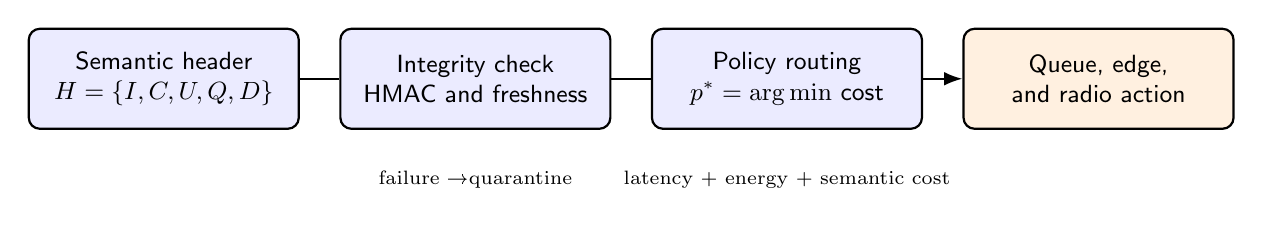
\begin{tikzpicture}[font=\sffamily\small, >=Latex, node distance=5mm and 5mm,
  box/.style={draw, rounded corners, align=center, minimum height=0.5in, minimum width=1.35in, fill=blue!8, thick},
  arrow/.style={->, thick}]
  \node[box] (header) {Semantic header\\$H=\{I,C,U,Q,D\}$};
  \node[box, right=of header] (verify) {Integrity check\\HMAC and freshness};
  \node[box, right=of verify] (route) {Policy routing\\$p^*=\arg\min$ cost};
  \node[box, right=of route, fill=orange!12] (action) {Queue, edge,\\and radio action};
  \draw[arrow] (header) -- (verify) -- (route) -- (action);
  \node[below=4mm of verify, align=center, font=\scriptsize] {failure \textrightarrow quarantine};
  \node[below=4mm of route, align=center, font=\scriptsize] {latency + energy + semantic cost};
\end{tikzpicture}
\end{document}
